\documentclass[10pt]{article}
\usepackage{amssymb,amsmath,graphicx,color,multicol,mycommands}
\usepackage{amsfonts}
\newcommand{\bbR}{{\mathbb R}}
\newcommand{\bbZ}{{\mathbb Z}}
\newcommand{\bbS}{{\mathcal S}}
\newcommand{\bbK}{{\mathcal K}}
\newcommand{\bbV}{{\mathcal V}}
\newcommand{\bbI}{{\mathcal I}}
\newcommand{\bbC}{{\mathcal C}}
\newcommand{\bbL}{{\mathcal L}}
\newcommand{\remove}[1]{}
\usepackage{epsfig,latexsym,graphicx}
\setlength{\textwidth}{17cm}
\setlength{\textheight}{23cm}
\setlength{\oddsidemargin}{5pt}
\setlength{\evensidemargin}{5pt}
\setlength{\topmargin}{-0.05in}
\newtheorem{observation}{Observation}
\newtheorem{fact}{\noindent {\bf Fact}}

\begin{document}
\begin{multicols}{2}
\section{Simulation}
We consider multiple simulation scenarios and in each one we compare the performances of projection quantiles (PQ) as well as its weighted version, i.e. WPQ. WPQ profiles are calculated using the above algorithm to obtain 90\% coverage sets in all direction, and the tuning parameter values are fixed at: $k=100, a=0.5, b=0.2$ and $\epsilon=0.9$.

\paragraph{}In figure 1 we present comparison of weighted (right panel) and unweighted (left panel) versions of projection quantiles from 4 simulated datasets, which have been taken from bivariate distributions for the sake of visualization.

\paragraph{Setup 1: Bivariate Normal}The bivariate random variable $(X_1,X_2)'$ considered here is
$$ \left(\begin{matrix}
X_1 \\ X_2
\end{matrix}\right) \quad\sim\quad \mathcal{N}_2\left(
\left(\begin{matrix}
0 \\ 0
\end{matrix}\right),
\left(\begin{matrix}
1 & 0.5 \\ 0.5 & 1
\end{matrix}\right)\right) $$
We generate 5000 independent draws from this distribution. Alongwith the PQ and WPQ profiles, we also plot the 90\% confidence ellipsoid for the sake of comparison.

\paragraph{Setup 2: Symmetric Normal mixture}Here we consider a 1:1 mixture of Two bivariate normal distributions, $\mathcal{N}_2((2,0)',\bfSigma_1)$ and $\mathcal{N}_2((-2,0)',\bfSigma_2)$, with
$$\bfSigma_1 = \left(\begin{matrix}
1 & 0.5 \\ 0.5 & 1
\end{matrix}\right),
\bfSigma_2 = \left(\begin{matrix}
1 & -0.5 \\ -0.5 & 1
\end{matrix}\right)$$
We draw 5000 samples from each distribution and compute 90\% PQ and WPQ for the mixture data.

\paragraph{Setup 3: Asymmetric Normal mixture}We keep the first distribution same as above, but change the second distribution to have a mean $(-1,0)'$ and covariance matrix $0.3\bfSigma_2$. We draw 5000 and 2000 samples from these distributions respectively, which gives the data-cloud an asymmetric butterfly shape.

\paragraph{Setup 4: Dependent exponential distribution}We take $X_1$ and $X_2$ distributed as $Exp(1)$ and the dependency structure between the two variables is specified by a Gaussian copula with correlation parameter $0,5$.

\paragraph{Observations}
\begin{enumerate}
\item In the first setup (Fig. 1, panels a and b) the WPQ profiles are almost identical to the confidence ellipsoids, while the PQ coverage sets severely underestimate actual confidence regions.
\item In setups 2 and 3 (panels c/d and e/f), weighted projection quantiles capture the shape of the data cloud in a much better fashion.
\item Coverage areas of PQ profiles are always less than those of corresponding WPQ profiles.
\item For coverage sets at lower probability values, the curves in the WPQ profiles cross themselves. We do not see this 'looping' for higher quantile values.
\end{enumerate}
\end{multicols}

\begin{figure}[t]
	\centering
		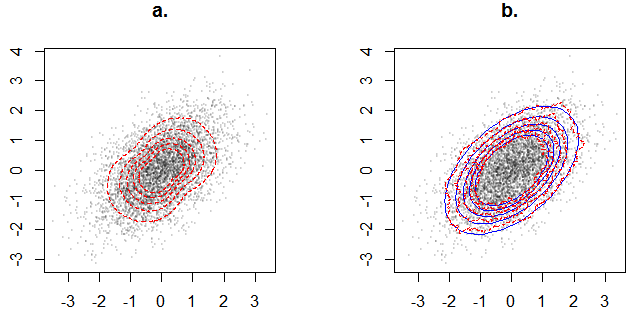
\includegraphics[height=5cm]{Sim_bvn.png}\\
		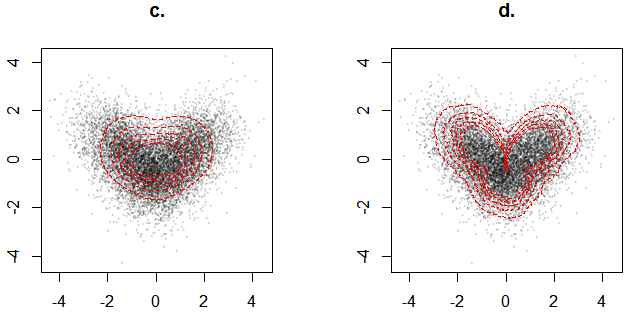
\includegraphics[height=5cm]{Sim_mixsym.png}\\
		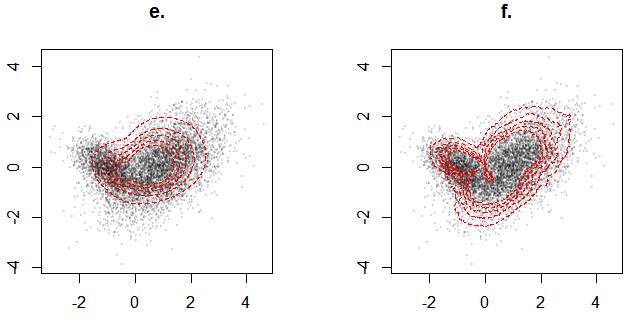
\includegraphics[height=5cm]{Sim_mixasym.png}\\
		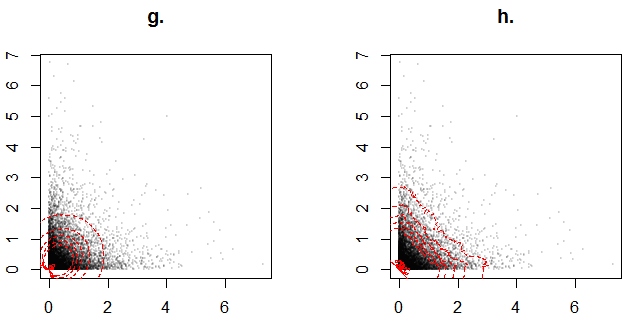
\includegraphics[height=5cm]{Sim_exp2.png}
	\label{fig:fig1}
	\caption{(Left) PQ and (Right) WPQ profiles for the four simulation scenarios. Blue lines in panel b represent actual confidence ellipsoids}
\end{figure}
\end{document}